\documentclass[ignorenonframetext,]{beamer}
\setbeamertemplate{caption}[numbered]
\setbeamertemplate{caption label separator}{: }
\setbeamercolor{caption name}{fg=normal text.fg}
\beamertemplatenavigationsymbolsempty
\usepackage{lmodern}
\usepackage{amssymb,amsmath}
\usepackage{ifxetex,ifluatex}
\usepackage{fixltx2e} % provides \textsubscript
\ifnum 0\ifxetex 1\fi\ifluatex 1\fi=0 % if pdftex
\usepackage[T1]{fontenc}
\usepackage[utf8]{inputenc}
\else % if luatex or xelatex
\ifxetex
\usepackage{mathspec}
\else
\usepackage{fontspec}
\fi
\defaultfontfeatures{Ligatures=TeX,Scale=MatchLowercase}
\fi
% use upquote if available, for straight quotes in verbatim environments
\IfFileExists{upquote.sty}{\usepackage{upquote}}{}
% use microtype if available
\IfFileExists{microtype.sty}{%
\usepackage{microtype}
\UseMicrotypeSet[protrusion]{basicmath} % disable protrusion for tt fonts
}{}
\newif\ifbibliography
\usepackage{graphicx,grffile}
\makeatletter
\def\maxwidth{\ifdim\Gin@nat@width>\linewidth\linewidth\else\Gin@nat@width\fi}
\def\maxheight{\ifdim\Gin@nat@height>\textheight0.8\textheight\else\Gin@nat@height\fi}
\makeatother
% Scale images if necessary, so that they will not overflow the page
% margins by default, and it is still possible to overwrite the defaults
% using explicit options in \includegraphics[width, height, ...]{}
\setkeys{Gin}{width=\maxwidth,height=\maxheight,keepaspectratio}

% Prevent slide breaks in the middle of a paragraph:
\widowpenalties 1 10000
\raggedbottom

\AtBeginPart{
\let\insertpartnumber\relax
\let\partname\relax
\frame{\partpage}
}
\AtBeginSection{
\ifbibliography
\else
\let\insertsectionnumber\relax
\let\sectionname\relax
\frame{\sectionpage}
\fi
}
\AtBeginSubsection{
\let\insertsubsectionnumber\relax
\let\subsectionname\relax
\frame{\subsectionpage}
}

\setlength{\parindent}{0pt}
\setlength{\parskip}{6pt plus 2pt minus 1pt}
\setlength{\emergencystretch}{3em}  % prevent overfull lines
\providecommand{\tightlist}{%
\setlength{\itemsep}{0pt}\setlength{\parskip}{0pt}}
\setcounter{secnumdepth}{0}

\title{Datenbanken}
\author{Jan-Philipp Kolb}
\date{21 April 2017}

\begin{document}
\frame{\titlepage}

\begin{frame}{\href{https://de.wikipedia.org/wiki/Datenbank}{Was sind
Datenbanken?}}

\begin{itemize}
\tightlist
\item
  Eine Datenbank, auch Datenbanksystem (DBS) genannt, ist ein System zur
  elektronischen Datenverwaltung.
\item
  Die wesentliche Aufgabe eines DBS ist es, große Datenmengen effizient,
  widerspruchsfrei und dauerhaft zu speichern.
\end{itemize}

\end{frame}

\begin{frame}{\href{https://cran.r-project.org/web/packages/dplyr/vignettes/databases.html}{Wann
sollte man R um Datenbanken ergänzen?}}

\begin{itemize}
\tightlist
\item
  Wenn ein Datensatz in den Arbeitsspeicher passt, gibt es keinen Grund
  eine Datenbank zu nutzen.
\end{itemize}

Man nutzt die Schnittstelle zu Datenbanken,\ldots{}

\begin{itemize}
\tightlist
\item
  weil die Daten bereits in einer Datenbank vorgehalten werden
\item
  oder weil der Datensatz nicht in den Arbeitsspeicher passt
\end{itemize}

\end{frame}

\begin{frame}{Die drei großen Open-Source Datenbanken}

\begin{itemize}
\tightlist
\item
  sqlite, mysql and postgresql
\item
  für alle drei gibt es Anbindungen in R
\item
  und auf diese Anbindungen soll in der Folge der Fokus liegen
\end{itemize}

\end{frame}

\begin{frame}{\href{https://www.r-bloggers.com/database-interfaces/}{Was
ist der Unterschied zwischen SQL und NoSQL}}

\begin{figure}[htbp]
\centering
\includegraphics{https://i2.wp.com/ropensci.org/assets/blog-images/2015-05-20-database-interfaces/databases_diagram.jpg?w=456}
\caption{}
\end{figure}

\end{frame}

\begin{frame}{\href{http://www.torsten-horn.de/techdocs/sql.htm}{Vergleich
zwischen MySQL und PostgreSQL}}

\begin{figure}[htbp]
\centering
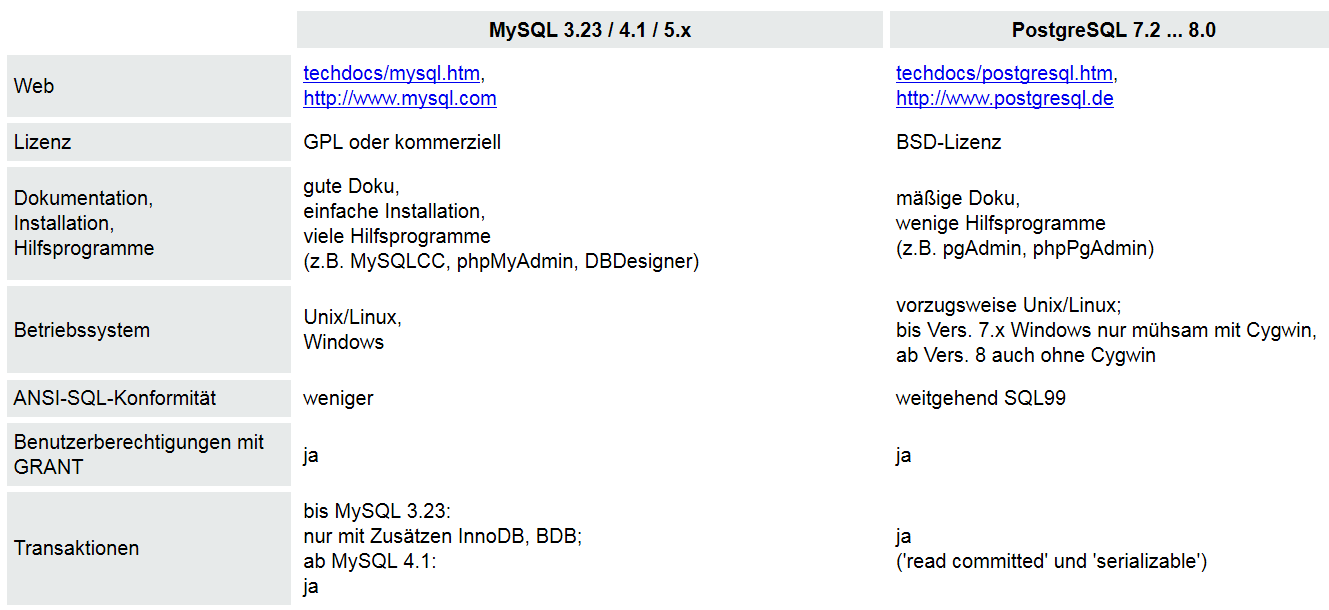
\includegraphics{figure/VergleichDatenbanken.PNG}
\caption{}
\end{figure}

\end{frame}

\begin{frame}{\href{http://www.statmethods.net/input/dbinterface.html}{Quick-R
zur Integration von Datenbanken}}

\begin{figure}[htbp]
\centering

\includegraphics{figure/quickr_AccessDatabases.PNG}
\caption{}
\end{figure}

\end{frame}

\begin{frame}[fragile]{CouchDB}

\begin{itemize}
\tightlist
\item
  \href{https://github.com/ropensci/sofa}{zur Interaktion mit CouchDB
  kann das Paket \texttt{sofa} verwendet werden}
\end{itemize}

\end{frame}

\begin{frame}{\href{https://cran.r-project.org/web/packages/RMySQL/index.html}{\texttt{RMySQL}}}

\end{frame}

\begin{frame}{Links}

\begin{itemize}
\item
  \href{https://cran.r-project.org/web/packages/dplyr/vignettes/databases.html}{Datenbanken
  in R}
\item
  \href{https://shiny.rstudio.com/articles/overview.html}{Database
  basics - dplyr and DBI}
\item
  \href{https://cran.r-project.org/web/packages/DBI/vignettes/DBI-proposal.html}{Frühe
  Entwicklung zu Integration von Datenbanken}
\end{itemize}

\end{frame}

\end{document}
